\subsection{Inverse Problem} 
\label{sec:inverse}

Before attempting solving the inverse problem,
we need to make sure that the observed data are
comparable to the simulated one.
To this end, Figure~\ref{fig:compare}
compares PC mean water surface elevation profiles
with their counterparts from the observed gauge locations.
The plots show good agreement between the simulations and the observations at different
locations and at different times. 
%
\begin{figure}[h]
\begin{tabular}{clc}
%        
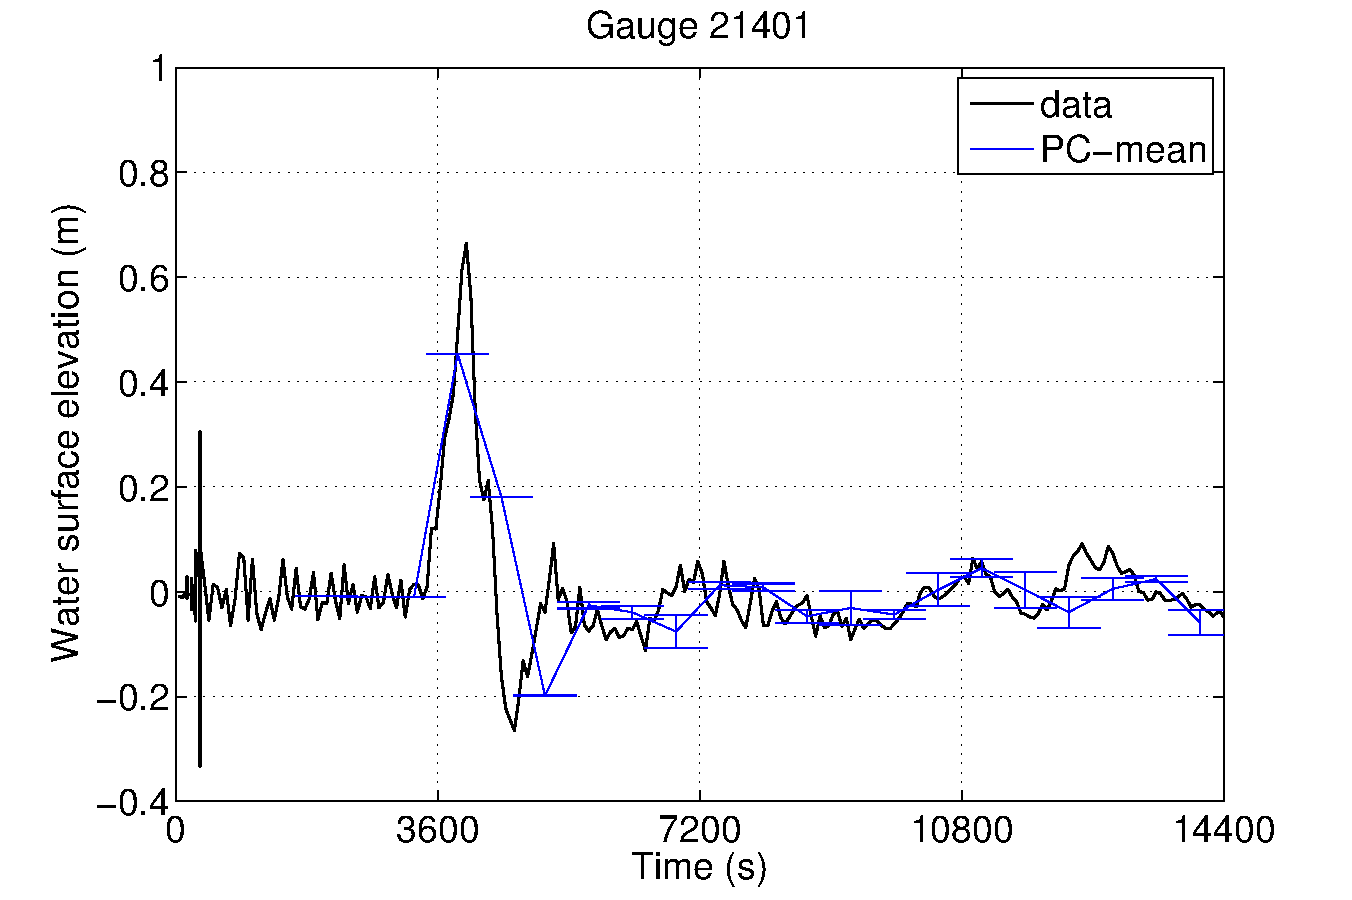
\includegraphics[width=0.475\textwidth]{../figures/compare1.pdf} &
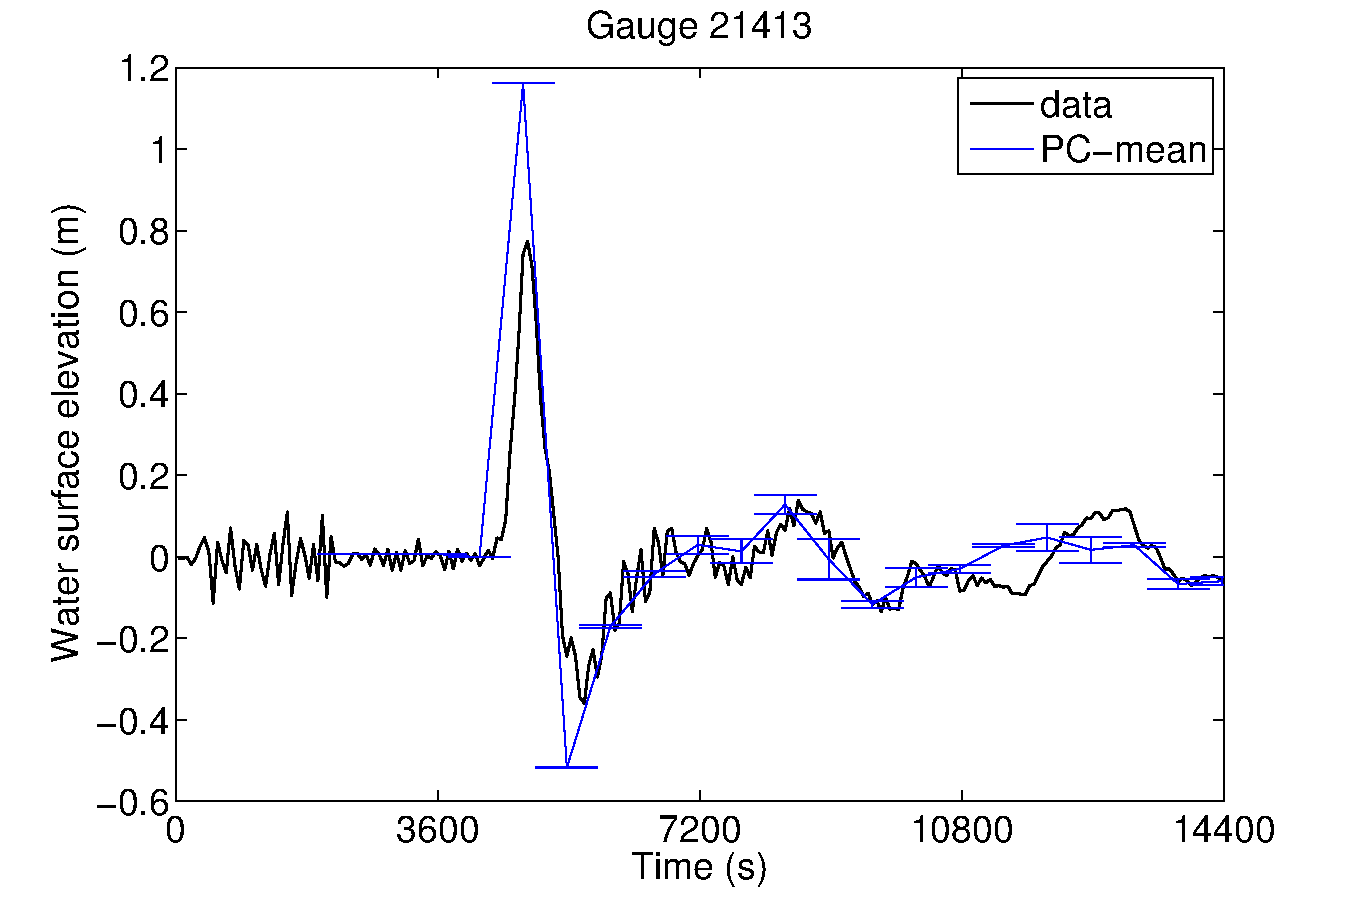
\includegraphics[width=0.475\textwidth]{../figures/compare2.pdf} \\
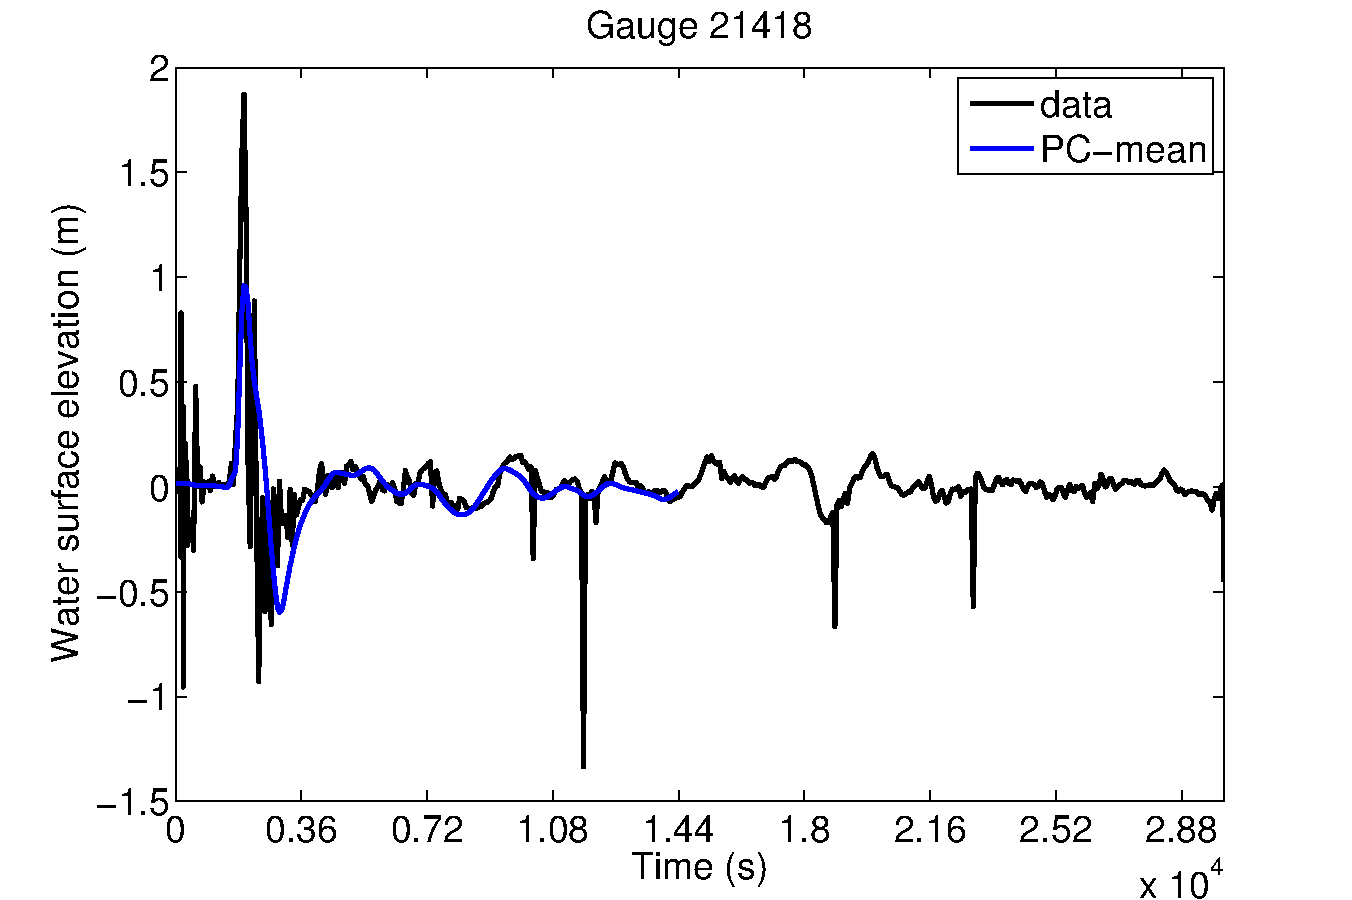
\includegraphics[width=0.475\textwidth]{../figures/compare3.pdf} &
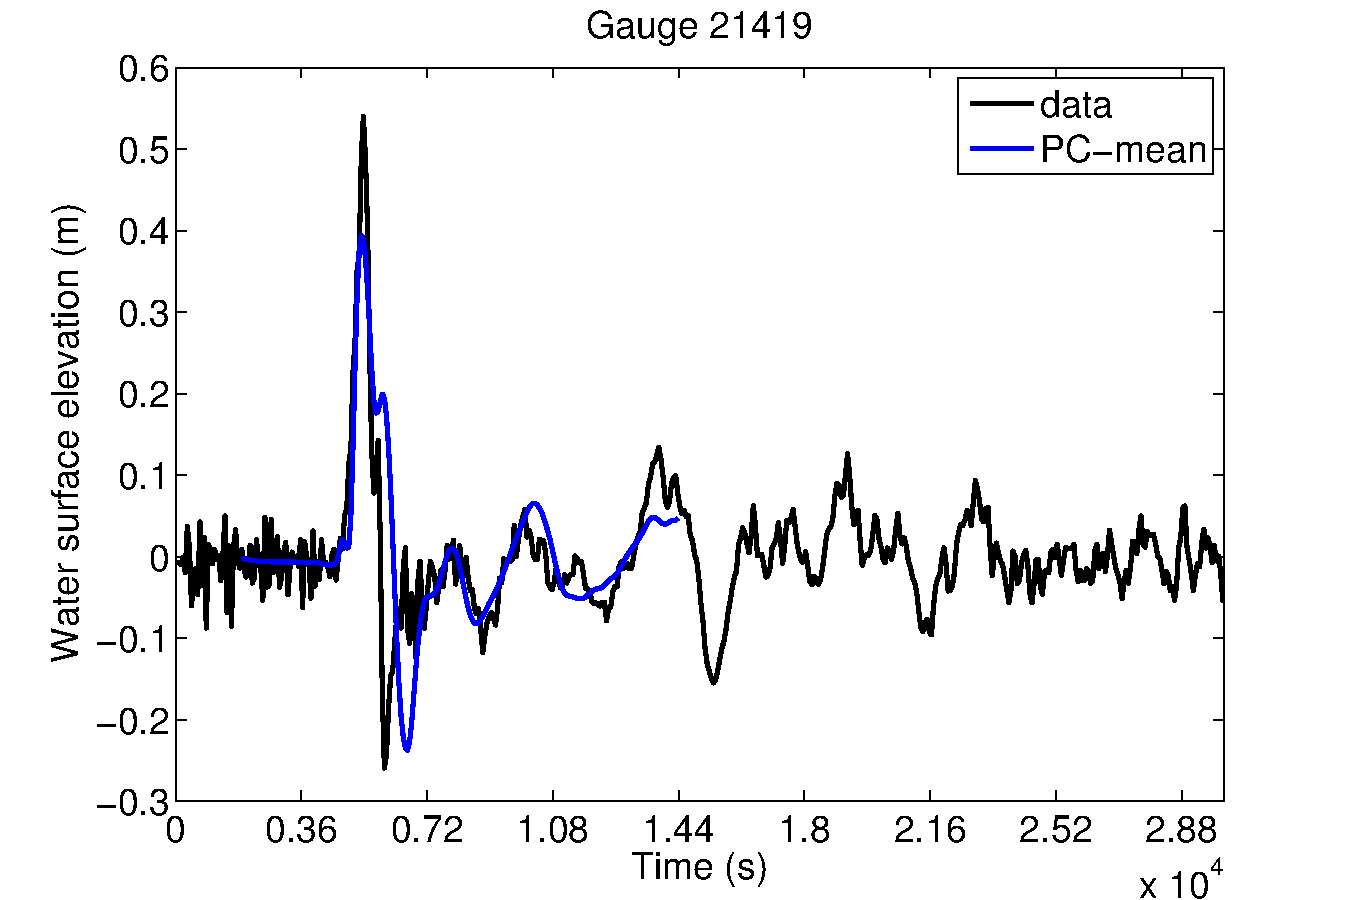
\includegraphics[width=0.475\textwidth]{../figures/compare4.pdf}
\end{tabular}
\caption{Comparison of PC mean 
and observed data of water surface elevation with time at the four gauges.}
\label{fig:compare}
\end{figure}     

Figure~\ref{fig:compare} can be recast as a scatter plot shown in 
Figure~\ref{fig:scatter}.
\begin{figure}[h]
\centering
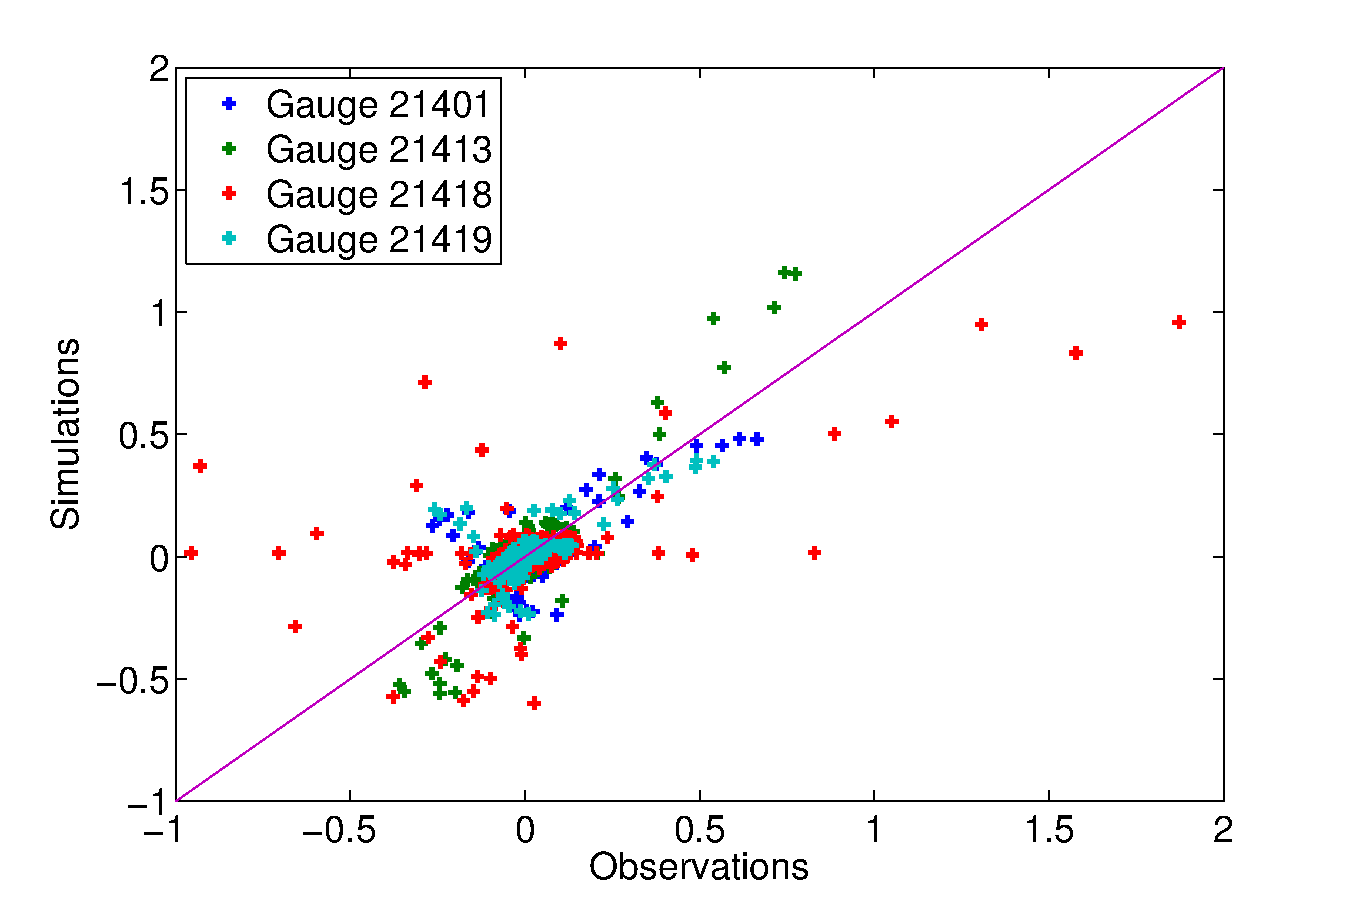
\includegraphics[width=0.475\textwidth]{../figures/scatter.pdf} 
\caption{Scatter plot of PC mean water surface elevation vs. observed ones.}
\label{fig:scatter}

\end{figure}        

We now can exploit the surrogate model in the Bayesian inference of the Manning's 
roughness coefficient.  To this end, an adaptive MCMC method is used to sample 
the posterior distributions \citep{Gareth2009,Haario2001} and consequently 
update the Manning's roughness coefficient distributions in light of the 
observed data. This sampling, demanding tens of thousands of forward simulations, 
would have been prohibitively expensive in the
absence of the surrogate, as the generation of each sample would have required an
independent Geoclaw realization. The surrogate provides a computationally
efficient alternative, and requires only evaluating the PCE for different values 
of the seed $\xxi$. The setup of the Bayesian inference problem,
MCMC chains for the input drag parameters and the corresponding posterior distributions are 
presented and discussed in this section. 




The observed data collected at different locations 
in the likelihood function (Equation~\ref{eq:likelihood}) to update the input parameters.
MCMCs of $40,000$ iterations are obtained for the Manning roughness coefficients: 
$N_1$,$N_2$ and $N_3$ as well as for the variance $\sigma^2$. Figure \ref{fig:mcmc} 
shows the sample chains for
the input parameters for different iterates of the MCMC algorithms. 
The different panels
shows well-mixed chains for all parameters.
However, all chains span the entire range
of the prior, and so it appears that the observations are not informative 
concerning this uncertain input.  $N_{2}$ chain appears to be concentrated in the lower end of the
parameter range, with values between 0.005 and 0.1.
The chain for the variance is also shown in 
Figure \ref{fig:mcmc} and appears to be well mixed.


\begin{figure}[h]
\begin{tabular}{clc}
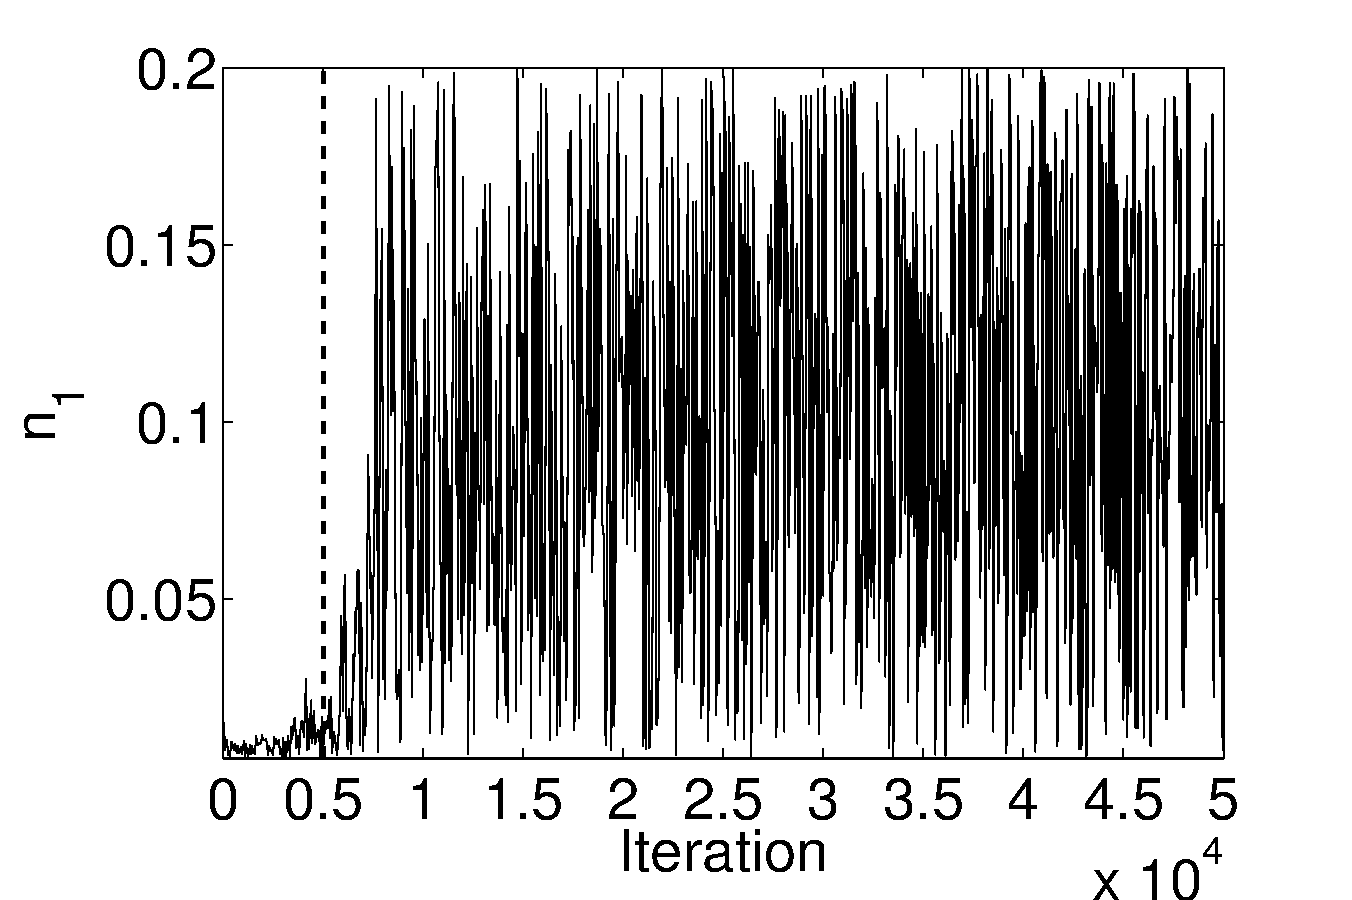
\includegraphics[width=0.475\textwidth]{../figures/chain_p1.pdf} &
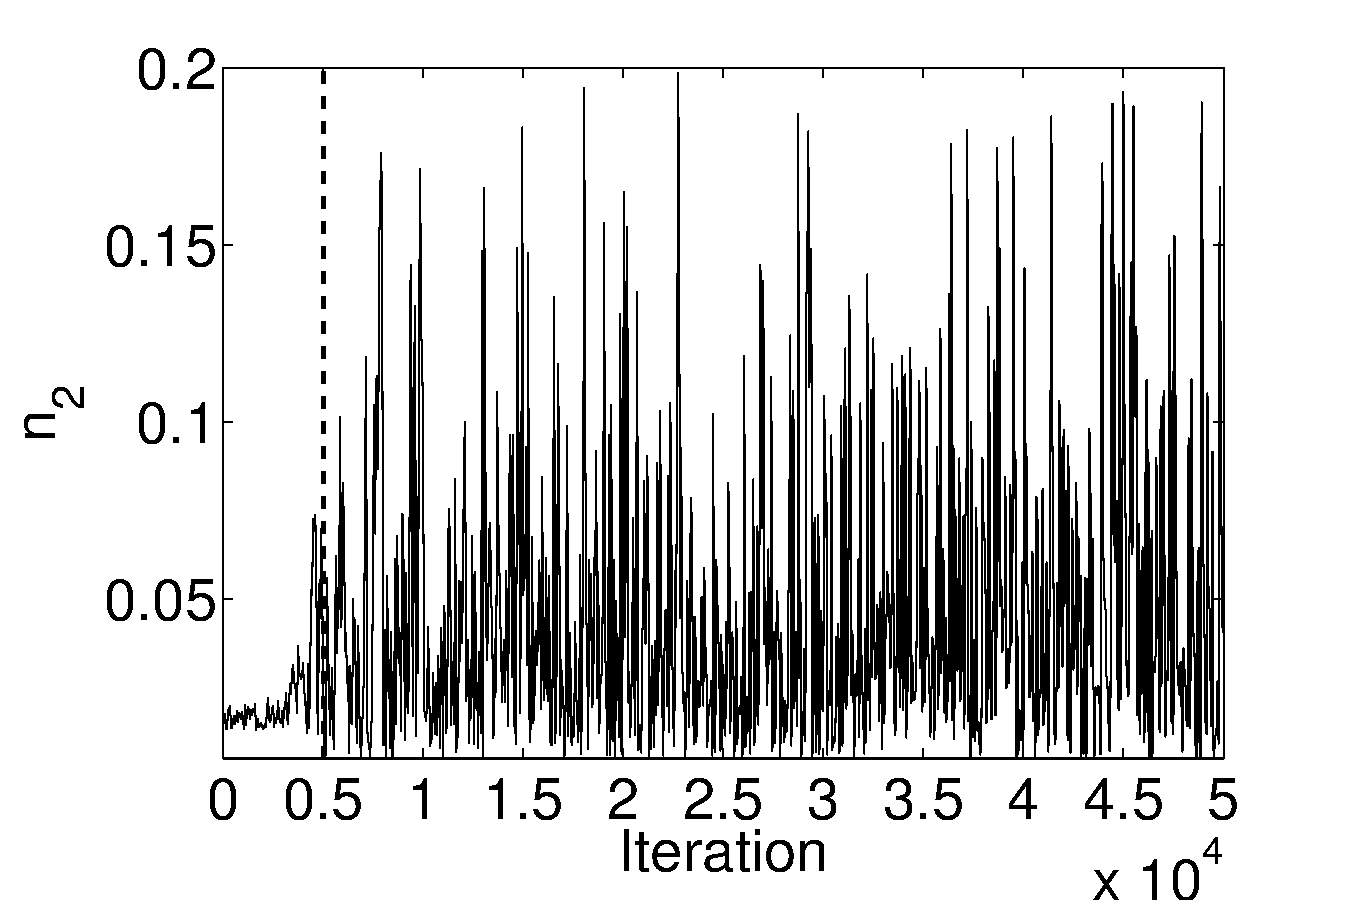
\includegraphics[width=0.475\textwidth]{../figures/chain_p2.pdf} \\
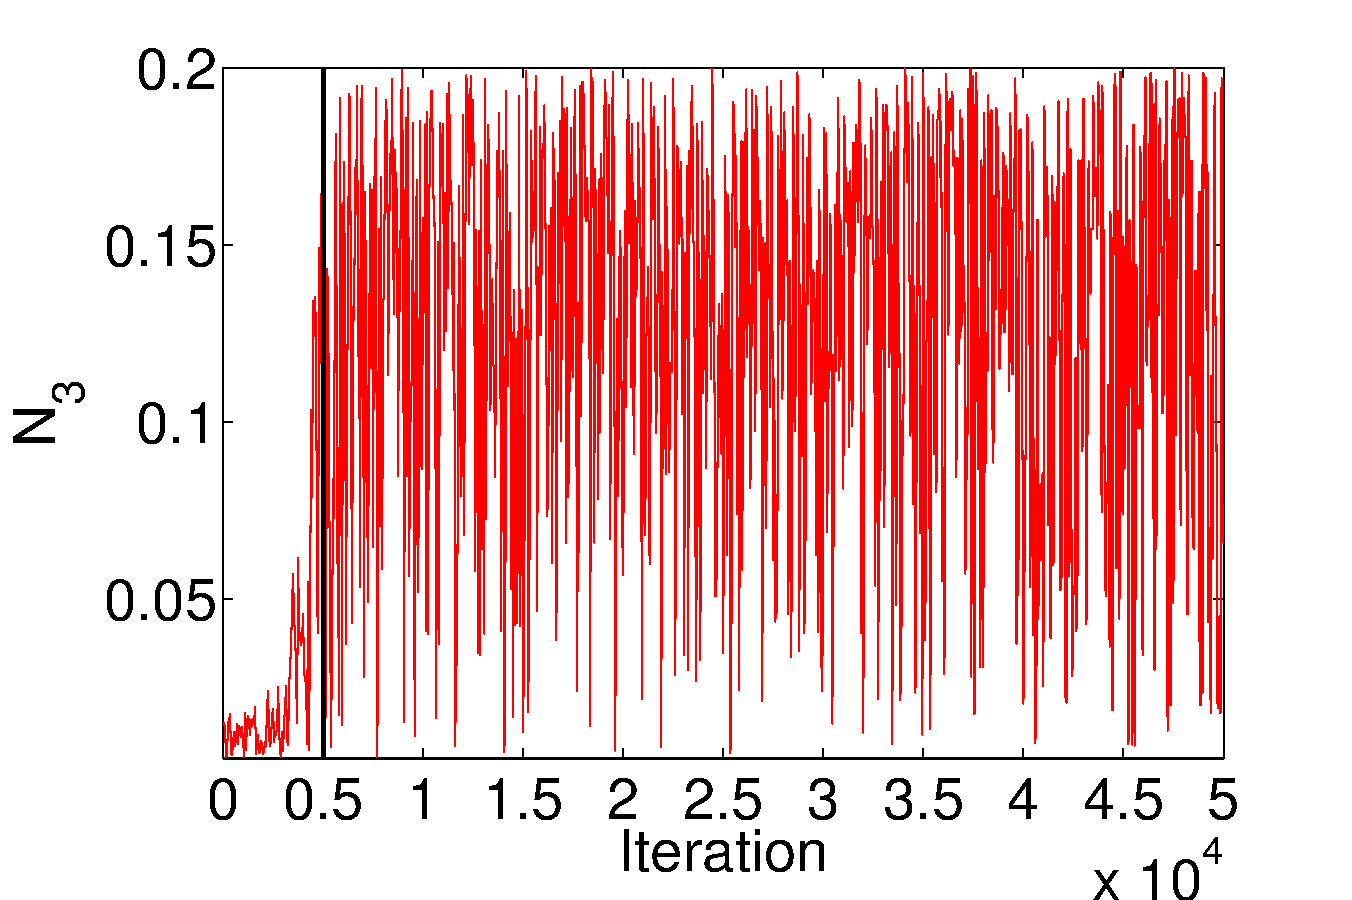
\includegraphics[width=0.475\textwidth]{../figures/chain_p3.pdf} &
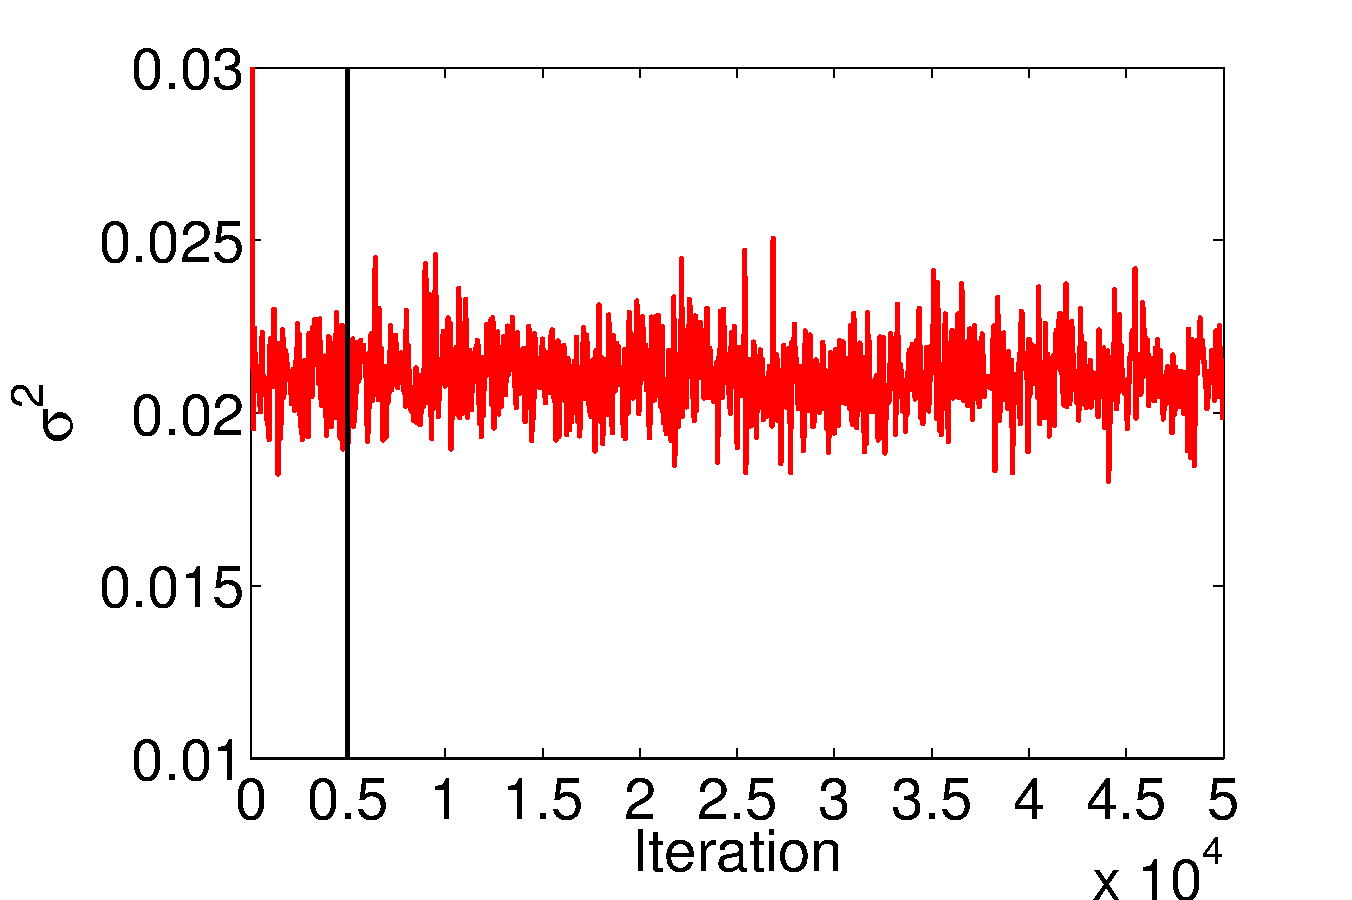
\includegraphics[width=0.475\textwidth]{../figures/chain_s1.pdf}
\end{tabular}
\caption{Chain samples for the three Manning's roughness coefficients $N_1,N_2,N_3$ and $\sigma^2$
the variance between simulations and observations.}
\label{fig:mcmc} 
\end{figure}

The computed MCMC chains can be readily used to determine the posterior 
distribution; kernel density estimation (KDE) is used for this purpose
~\citep{Parzen1962,Silverman1986}(The first 6000 iterates, associated 
with the burn-in period, are discarded). The resulting posterior pdfs 
of the three Manning's roughness coefficients $N_1,N_2,N_3$ are shown 
in Figure~\ref{fig:pdfs}.  As expected from the chains shown in Figure
~\ref{fig:mcmc}, the posterior pdf of $N_2$, exhibits well-defined peak, 
with a Maximum A Posteriori (MAP) estimate of around 0.013; an extended tail 
towards the higher Manning's roughness coefficient values is also observed.
In contrast, the posterior pdfs of $N_1$ and $N_3$ appear to be fairly flat, 
and similar to the uniform prior. This is an indication that 
the observed data were not useful to refine our prior knowledge for $N_1$ and $N_3$.  

The posterior distribution of the variance is also shown in Figure~\ref{fig:mcmc}. 
Taking the square root of the MAP values yields the water surface elevation standard 
deviation, and the latter is a reflection of the mismatch between the model and 
observed data estimated to be 0.144~$m$.

 \begin{figure}[h]
        \begin{tabular}{clc}
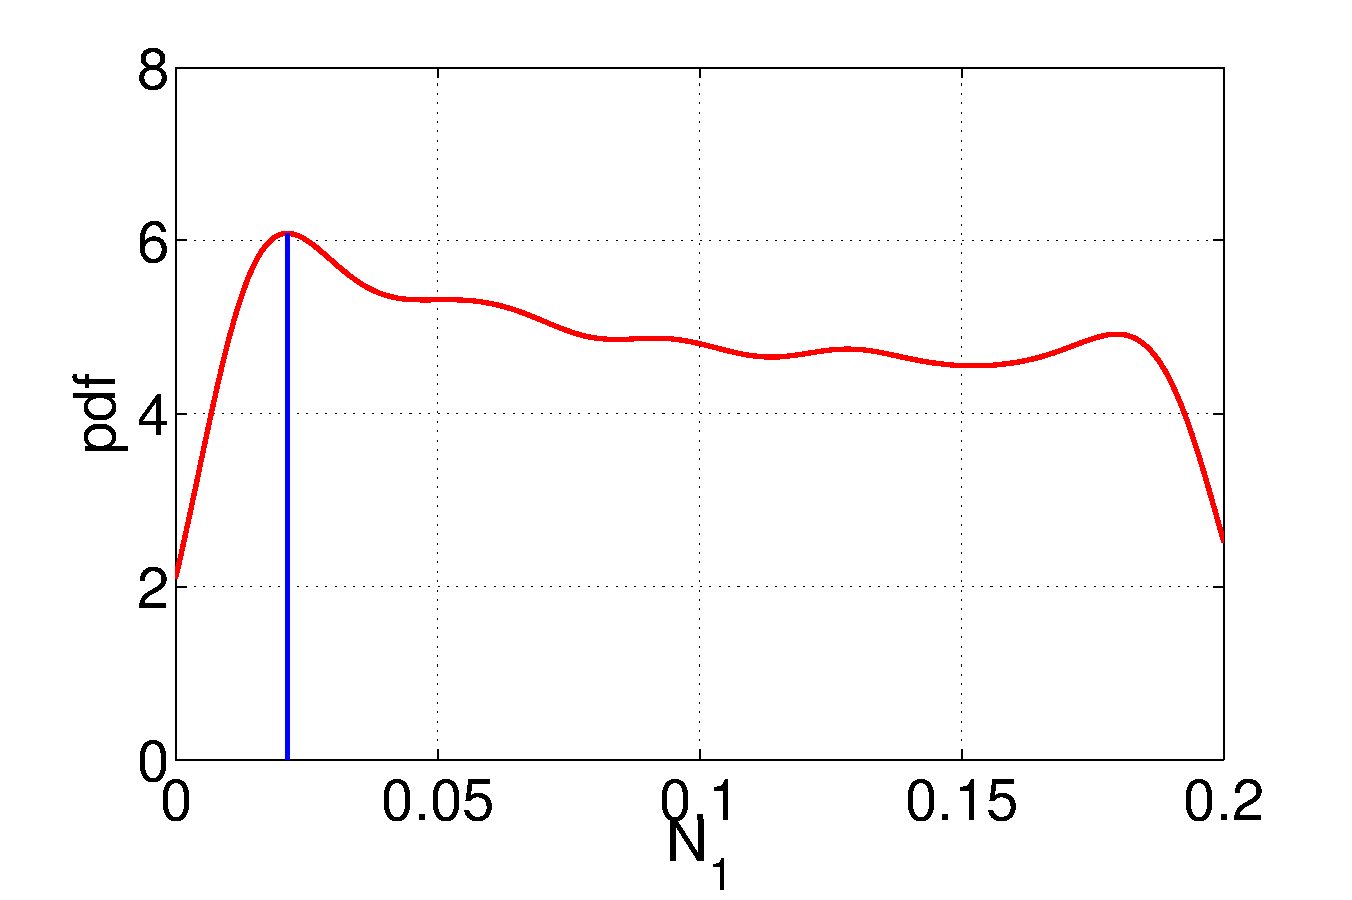
\includegraphics[width=0.475\textwidth]{../figures/pdf_p1.pdf} &
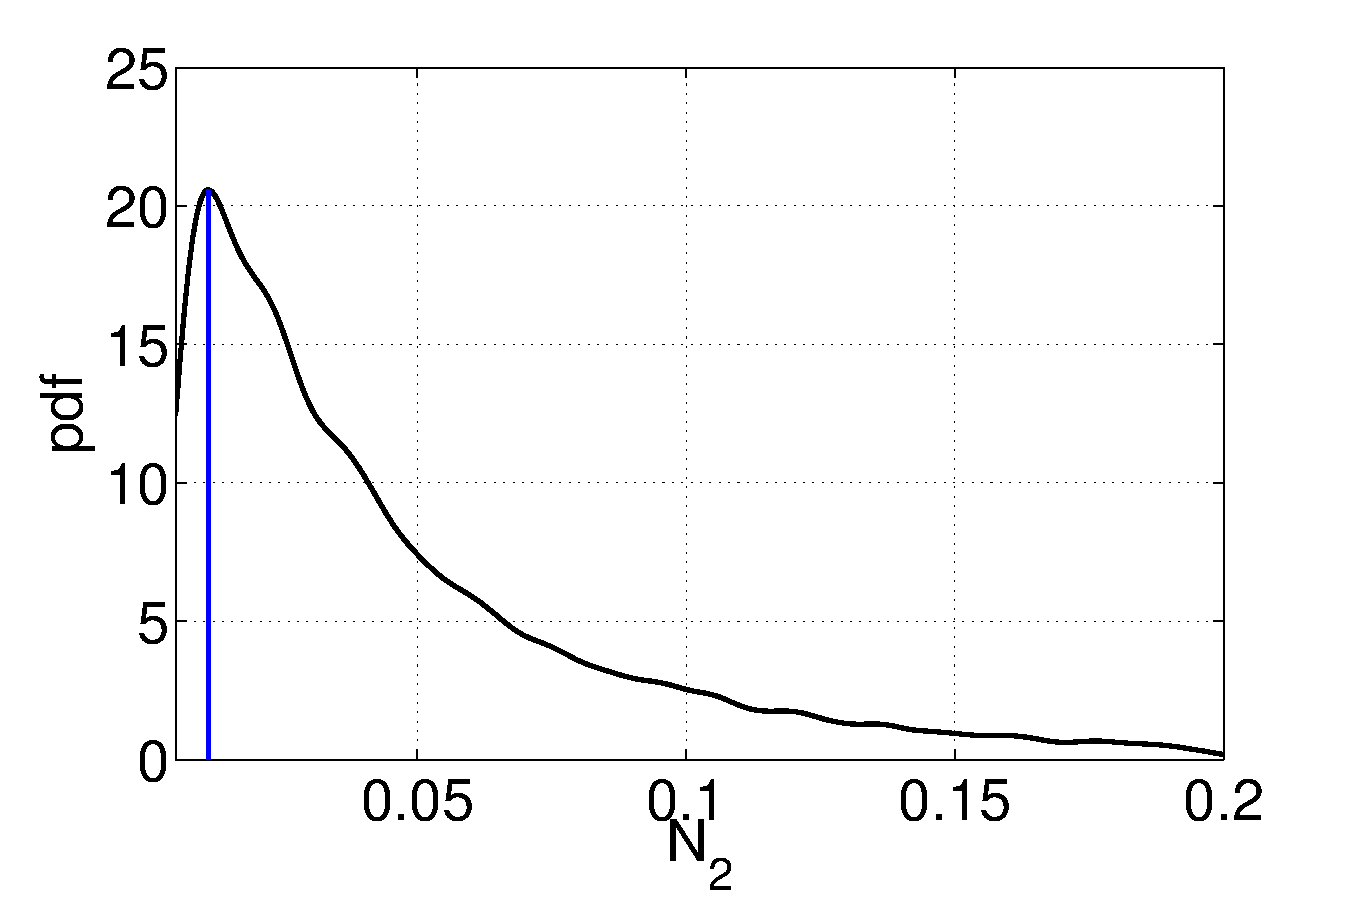
\includegraphics[width=0.475\textwidth]{../figures/pdf_p2.pdf} \\
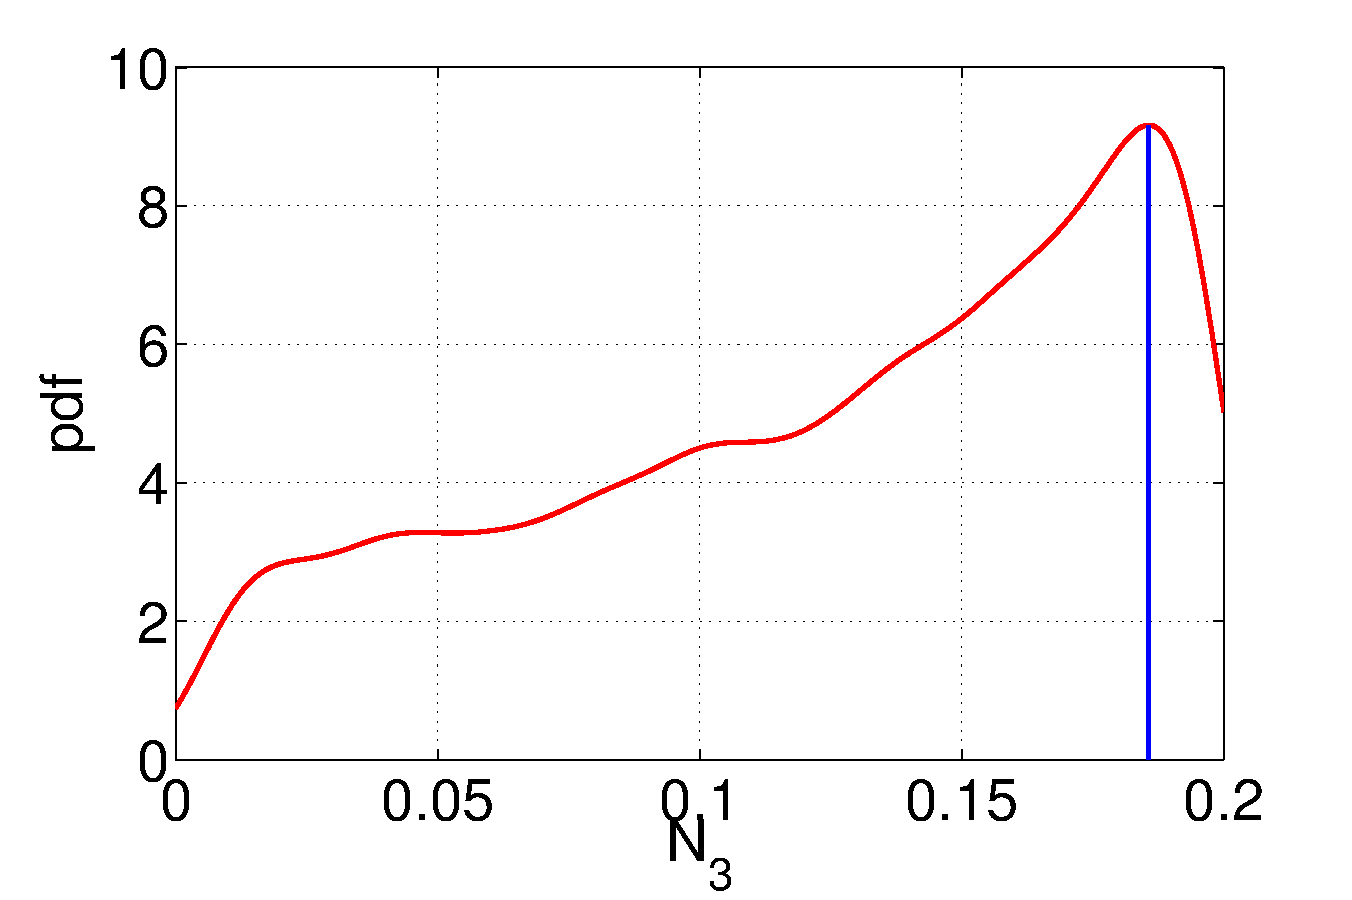
\includegraphics[width=0.475\textwidth]{../figures/pdf_p3.pdf} &
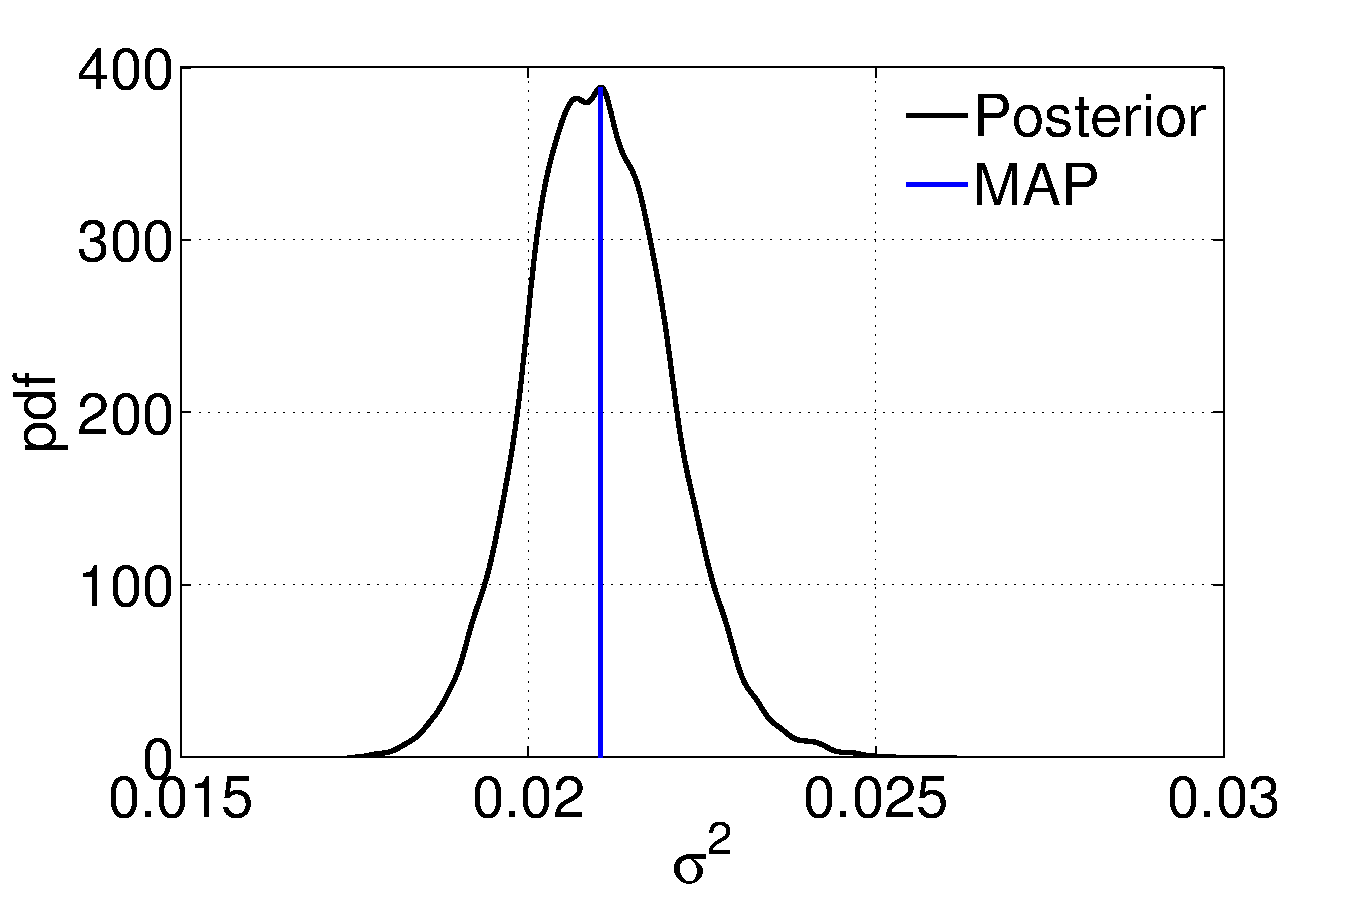
\includegraphics[width=0.475\textwidth]{../figures/pdf_s1.pdf}
        \end{tabular}
        \caption{Posterior distributions for the three Manning's roughness coefficients $N_1,N_2,N_3$ 
and $\sigma^2$ the variance between simulations and observations.}
\label{fig:pdfs} 
        \end{figure}
